\chapter{Review of Literature} \label{review-of-literature}

\section{Architecture} \label{Technology}

\subsection{Introduction} \label{subsec-lr-arc-intro}
\subsection{Summary} \label{subsec-lr-arc-summ}

\section{Technology} \label{Technology}

\subsection{Introduction} \label{subsec-lr-tech-intro}

The aim of this document is to review some of the state-of-the-art technology that can be used to architect the monitoring system for storing and handling big datasets and performing real-time analytics on them. The proposed architecture will consist of three layers: the batch layer, serving layer and speed layer.\\

\subsection{Batch Layer} \label{subsec-lr-batchlayer}

\subsubsection{test Introduction} \label{subsubsec-lr-batchlayer-intro}
A batch layer is required to store constantly growing big data and for historical data analysis that is used to identify patterns such as job failures, popular data, busy sites and so forth.  Many individuals consider Hadoop as the de facto framework for analysing big data. However, there are many technologies available in the distributed system such as the Internet that go beyond MapReduce, a programming model for processing big data that was introduced by Google \cite{mr-com} . In this chapter an attempt will be made to review such technologies.\\

\subsubsection{Apache Hadoop- MapReduce and HDFS} \label{subsubsec-lr-batchlayer-mr}
The Hadoop stack has been used for many research and commercial products. It has gone through rigorous implementation and testing, which makes it robust. There are many Hadoop ecosystems and distributions, but in order to make this review relevant to the proposed layer, the MapReduce and Hadoop Distributed File System (HDFS) will be analysed. MapReduce is a programming model that was designed to remove the complexity of processing data that are geographically scattered around the distributed infrastructure \cite{mr-com,mr-data}. It hides the complexity of computing in parallel, load balancing and fault tolerance over a large range of inter-connected machines from developers.\\

There are two simple parallel methods; map and reduce are predefined in the MapReduce programming model and are user-specified methods, so users have control over how the data should be processed \cite{mr-data}. Hadoop was designed taking into account that moving computing to where the data reside is better than vice versa as it will reduce bottlenecks in the network, especially when the data that are being transferred are at the rate of terabytes-to-petabytes \cite{mr-com}. Therefore, map and reduce jobs will be allocated to where the data reside, which will be scheduled by JobTask Manager as shown in Figure \ref{fig-map-reduce}. The data will be read from the local disk (file system); mapped, with all records being independently processed and key/value pairs assigned; intermediate results are stored to the local disk and they are shuffled (transferred to where the reduce jobs are located); and reduced, so that records with identical keys are processed together and the output is written back to the disk (this output could be an input to another MapReduce job) \cite{mr-com}. Fault tolerance in MapReduce is supported by periodically checking the heartbeat of the worker nodes, master failures can be protected against by using check-pointing, an approach used to enable applications to recover from failure.\\

\begin{figure}[H]
\centering
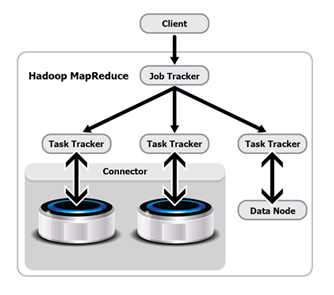
\includegraphics[width=0.5\textwidth]{Figures/map-reduce.png}
\caption{Hadoop Architecture}\label{fig-map-reduce}
\end{figure}

The MapReduce framework is built on HDFS and executes I/O operations on it. The HDFS guarantees: scalability on commodity hardware, fault tolerance, high throughput, load balance, data integrity and portability \cite{intro-hdfs}. It employs master-slave architecture, which is prone to single point failure. However, it facilitates failover to the standby server but this is prone to downtime. Data are replicated across disk nodes for load balancing, fault tolerance and high availability \cite{intro-hdfs}.

\subsection{Summary} \label{subsec-lr-tech-summ}